\documentclass{article}
\usepackage{geometry}
\usepackage{graphicx}
\usepackage{amsmath}
\usepackage{tikz}

\begin{document}

\title{WALT}
\author{Your Name}
\date{\today}

\maketitle

\section{Objective}

The objective of this project is to design, develop, and implement a wheeled quadruped robot capable of performing autonomous navigation in a controlled environment. The robot will integrate both walking and driving capabilities, allowing it to:

\begin{enumerate}
    \item Drive fully autonomously in a controlled environment from a start to an end point.
    \item Detect and avoid obstacles autonomously while maintaining a smooth path.
    \item Climb or overcome obstacles that hinder passing.
    \item Switch between driving and walking modes based on environmental conditions, such as encountering an obstacle that requires climbing.
\end{enumerate}

This project aims to combine real-time sensor data processing (e.g., LIDAR, cameras) with intelligent decision-making algorithms to allow the robot to autonomously navigate complex paths. Moreover, the robot has to be designed, and a sophisticated selection of the hardware components (such as servos, microcontroller, sensors, etc.) is necessary. Particular emphasis is placed on the development of a control system to manage locomotion and walking gaits, ensuring that all elements are combined effectively into a unified embedded system.

\subsection{Target Route}

The target route for the robot is designed to test its ability to navigate both driving and climbing modes in a structured environment. The route goes through a corridor, includes dynamic obstacle avoidance, and ends with a climbing task. Below is a detailed breakdown of the route and its key features:

\begin{enumerate}
    \item \textbf{Start:} The robot begins at the designated Start Point, located in a corridor.
    \item \textbf{Driving along the corridor:} The robot drives fully autonomously through the aisle and should be able to navigate past various obstacles.
    \item \textbf{Turning in the corridor:} After navigating the horizontal aisle, the robot should be able to navigate safely around a corner in the corridor.
    \item \textbf{Climbing an Obstacle:} To test and demonstrate the robot's climbing and walking capabilities, it will encounter an obstacle that requires a transition from driving mode to walking/climbing mode.
    \item \textbf{Goal:} After successfully completing the route, the robot reaches a predefined endpoint.
\end{enumerate}

This route evaluates the robot's capabilities in obstacle detection and avoidance, control and mechanical design, seamless transitions between driving and walking modes, and successfully overcoming challenges to reach the predefined endpoint.

\begin{figure}[h!]
    \centering
    \includegraphics[width=0.7\textwidth]{Paper/Target_Route.jpg}
    \caption{Target route of the robot}
    \label{fig:Target_Route}
\end{figure}

\subsection{Real-World Application of the Project}

The quadruped robot is well-suited for a variety of real-world applications. It excels in autonomous delivery, particularly for last-mile logistics, where fast-paced driving on flat surfaces is required, but the ability to overcome obstacles, such as stairs or curbs, is essential. In industrial environments, such as factories and warehouses, the robot is ideal for navigating primarily flat surfaces at high speeds while still being capable of overcoming occasional obstacles, ensuring smooth and efficient operations. Its versatility makes it valuable in any environment where fast driving is the primary mode of transport, but the ability to switch to walking or climbing is mandatory to handle challenging obstacles.

\section{Project Structure and Task Allocation}

\begin{figure}[ht]
    \centering
    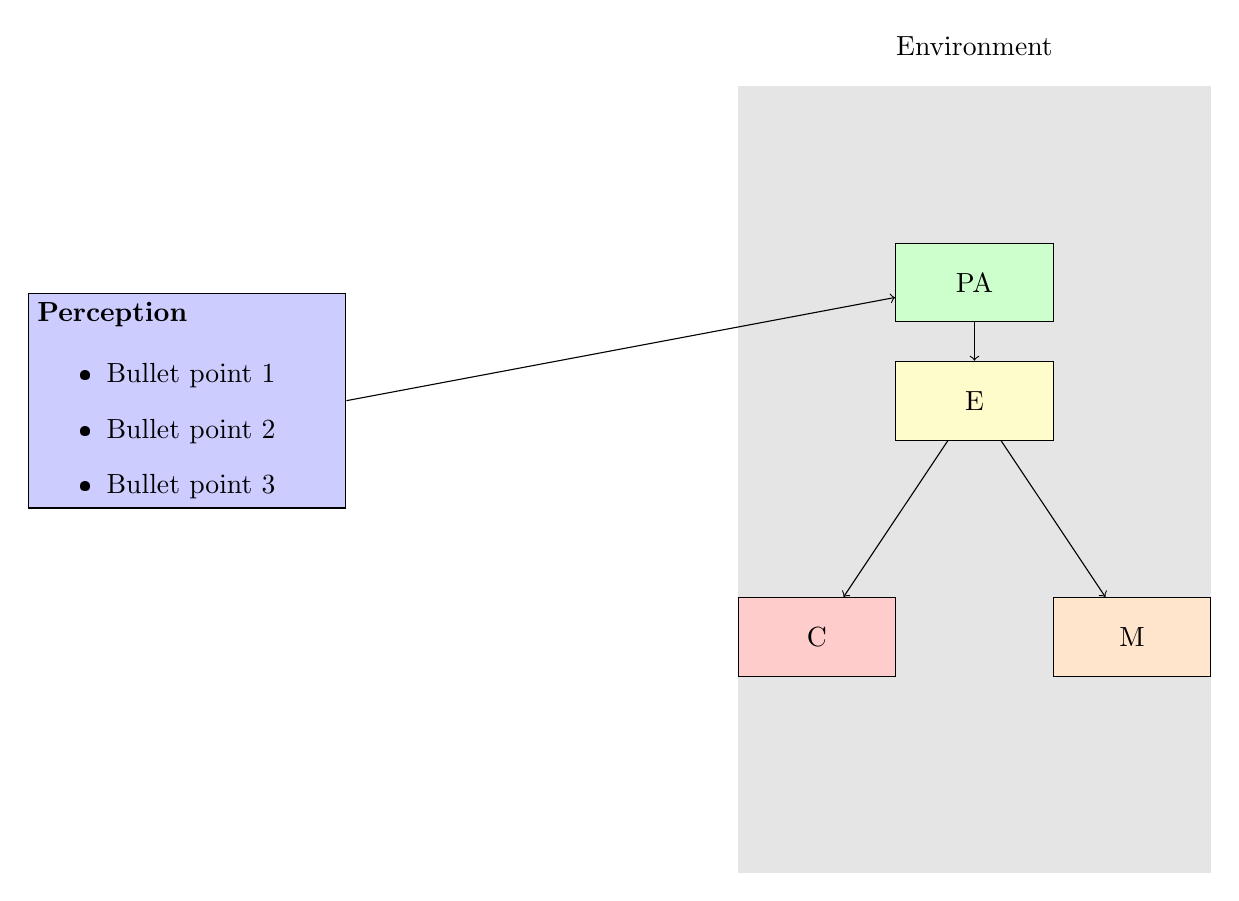
\begin{tikzpicture}
    % Large transparent rectangle representing environment
    \fill[gray!20] (-1, 4) rectangle (5, -6);

    % Label for the large environment rectangle
    \node at (2, 4.5) {Environment};

    % Perception:
    \node[draw, fill=blue!20, minimum width=4cm, minimum height=2cm, text width=3.8cm, align=left] (Perception) at (-8, 0) {
    \textbf{Perception} \\
    \begin{itemize}
        \item Bullet point 1
        \item Bullet point 2
        \item Bullet point 3
    \end{itemize}
    };
    
    \node[draw, fill=green!20, minimum width=2cm, minimum height=1cm] (PA) at (2, 1.5) {PA};
    \node[draw, fill=yellow!20, minimum width=2cm, minimum height=1cm] (E) at (2, 0) {E};

    % Rectangles outside the large environment
    \node[draw, fill=red!20, minimum width=2cm, minimum height=1cm] (C) at (0, -3) {C};
    \node[draw, fill=orange!20, minimum width=2cm, minimum height=1cm] (M) at (4, -3) {M};

    % Connections
    \draw[->] (Perception.east) -- (PA);
    \draw[->] (PA) -- (E);
    \draw[->] (E) -- (C);
    \draw[->] (E) -- (M);

    \end{tikzpicture}
    \caption{Project Structure}
    \label{fig:Project_Structure}
\end{figure}

\subsection{First Basic Design Ideas}

\subsubsection{Locomotion Mechanism}
Joints, servo mount positioning, etc.

\subsubsection{Mechanical Structure}
(TBD)

\subsubsection{Electronics and Embedded System}

\textbf{Microcontroller:} Raspberry Pi 5 8GB, powerful enough for the task.

\textbf{Camera:} Feed into Raspberry Pi; wireless/cable (Wi-Fi) feed to a laptop to run a vision algorithm and send back useful information for obstacle mapping.

\textbf{Power management:} (TBD)

\textbf{Obstacle Detection and Navigation:} ROS2 (Nav2) offers useful tools for sensors and processing.

\subsection{Control System}
ROS2 provides control packages useful for gaits and general control. 

\textit{Note:} ROS2 could be very beneficial for the system's architecture.


\end{document}
